\chapter{家族涂鸦}

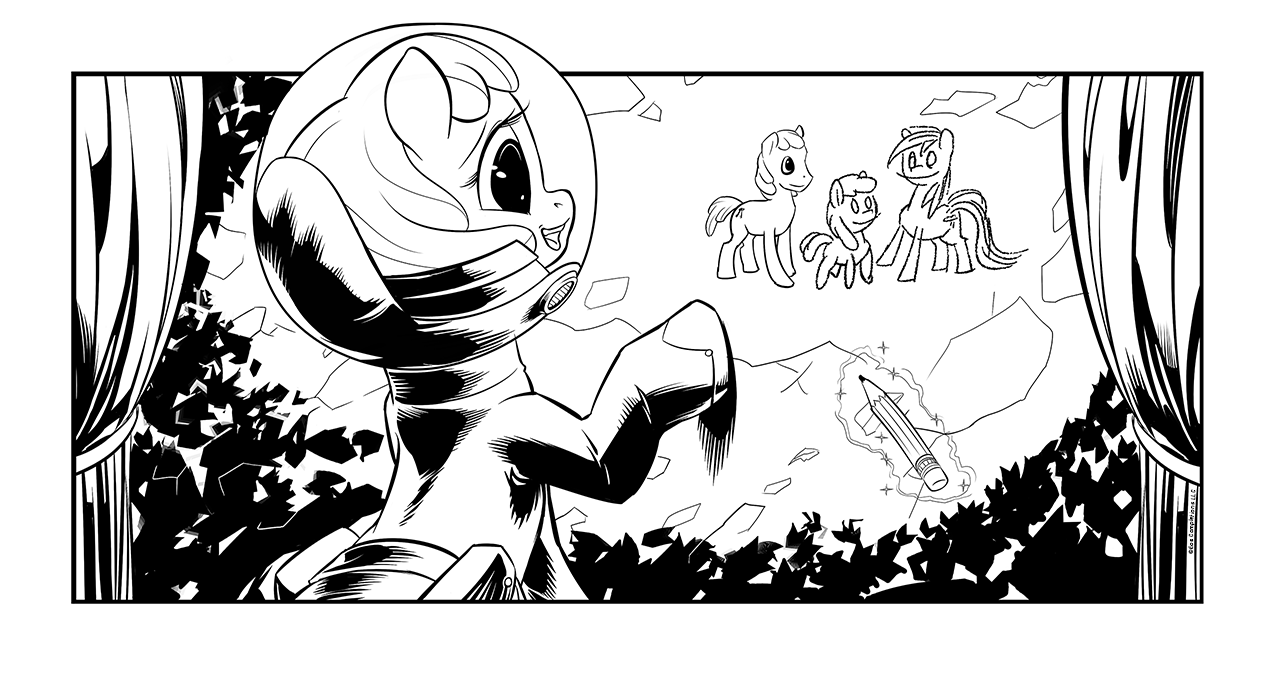
\includegraphics[width=0.9\linewidth]{image11.png}

\begin{intro}
你没有用电动工具,对吧?
\end{intro}

\daytimeplace{10}{1:30 PM}{铁锈庄园,52号国道中段}{Rust Manor, Big 52 SC Branch}

{\rt 嗯哼,大家下午好,这里是孤狼的铁锈庄园特别新闻!}

在噪杂的背景声之中可以清楚地听到一个女性的声音,然后有谁在叫着『你个老巫婆给我让座!』还有一阵金属撞击声。

{\rt DJ好货在新闻之后马上回来,我要说,什么叫好货啊,你在干什么,那是铁桌子,哦,哦,哦别!我对你够温柔的了,好吧,你自找的,尝尝我的爱与包容吧!}

在一阵被按住嘴的声音打断了放送之后,孤狼终于喘息着回到麦克风面前。

{\rt 代表好货祝你们健康,她很快回来,在她解开蹄子上的电线……好吧,我们还是来说我们的特别新闻!这个是来自一位铁锈庄园的电台同好!感谢小蝴蝶23!}

孤狼清了清喉咙然后继续往下讲。

{\rt 有些英雄倒下了,有些英雄被杀害了,有些英雄消失在避难厩中再也没回来……不过,我们的英雄被打屁股了,对,你没听错。在早上早些时候,小小幽灵在铁锈庄园外碰上了一队雇佣兵。一个卫兵当着很多小马的面骂了她。好吧,你这家伙脑子抽了么?我们知道这个孩子摧毁了赤兔领土上的那个农场,然后冲进重兵防守的隧道镇,那里的快乐扳机说她看到那个幼驹单枪匹马用一个石头砸坏了六个哨兵机器……但是你呢,你和一个小幼驹打架?你活得不耐烦了?就算现在你看起来打赢了那个小孩子——如果你管那叫做『打架』的话,在我看来不过是一个可爱的小雌驹想要对你示好却被你欺负得哭着跑开!}

然后是一阵长长的叹息。

{\rt 这就是所谓的感恩……L.P.播报结束,在好货回来之前先听点音乐吧,我先逃命了。保持优雅,52国道。}

然后是一阵音乐声。

\begin{music}
看着你步出一零零九房间

Saw you stretched out in room Ten O Nine

\medskip

你笑颜如花,却又泪眼潸然。

with a smile on your face and a tear right in your eye.

\medskip

那模糊的心意宛如雾里看花,

couldn't see to get a line on you,

\medskip

我甜蜜的爱侣啊。

my sweet honey love.
\end{music}

帕比躲在一辆废弃的卡车后面,依然抹着泪。这次她又做错什么了,她真的很努力去做一个好孩子,但是所有的事情看起来都和她对着干。从那个疯狂的派对机器马和房顶砸在头上开始——她就是块会吸引噩运的磁铁。妈妈为什么一直跑来跑去不等她?小小雌驹觉得又累又空虚。

\begin{music}
斑马的珠宝洒落在街上,

Zebra jewelry jangling down the street,

\medskip

你闭上眼睛,封闭心灵之窗。

make you shut your eyes at every filly that you meet.

\medskip

那冰封的心中仿佛风雪飘扬,

couldn't seem to get a high on you,

\medskip

我甜蜜的爱侣啊。

my sweet honey love.
\end{music}

但是帕比不能就这样坐下放弃!就算长路漫漫没有尽头,她的妈妈一定在山另一边的某处,或者就在下一座山后面,一次翻越一座山,总会找到妈妈的!

\begin{music}
愿公主为你降下一缕阳光,

May Celestia shine a light on you,

\medskip

优美的歌为你唱响。

make every song your favorite tune.

\medskip

愿公主为你降下一缕阳光,

may Celestia shine a light on you,

\medskip

温暖如傍晚的夕阳。

warm like the evening Sun.
\end{music}

黄色的小雌驹站了起来,在车子后面哭鼻子可没法找到妈妈,她是肩负重任的好孩子,不要在意那些小事,前进吧帕比!

\horizonline

\daytimeplace{10}{1:45 PM}{铁锈庄园,52号国道中段}{Rust Manor, Big 52 SC Branch}

在大门站岗的两个卫兵快速对视了一眼,看起来不确定该由谁应付这个走过来的幼驹。终于比较大的那个说话了,「抱歉小鬼,如果你想进去的话,你应该付钱,两百个瓶盖,还要把你的武器放在这里。」

帕比皱了皱眉头,两百对于她来说是个超级大的数字,她可以用自己的蹄子数到四,说不定还能数到十,不过两百?一百是多少?

「呃……我只是在找妈妈,超超拜托……」

「拿出你的瓶盖就行了,小孩子。」卫兵打了个哈切,想要保持冷静,但是他担心如果小雌驹没有钱还要往里走的话,或许该是叫老大……{}

「袋子!」

一个超级大的袋子飘在了帕比面前,她交给了卫兵,「呃……你们能帮我数数看么,这些闪亮瓶盖够么?」

卫兵点了点头然后把袋子倒在桌子上,那里面一多半是瓶盖,剩下的都是站前货币,甚至还有一些金币,「没问题,这些足够了。」那个卫兵看了看另一个守卫,而后者满脸失望地哼了一声,「你想干啥,这么可爱的一个小雌驹,你不会是认真的吧!」

那个卫兵叹了口气,数了两百个瓶盖,然后把剩下的还给帕比,小雌驹开心地把自己的收藏品收了起来。

「漂漂卫兵超超超谢谢你们!」

在城墙里面,铁锈庄园又小又拥挤,天空马车的残骸不但用来建造城墙,还被当做房子和商店,只在中间留出勉强够小马通行的小路,帕比觉得这里就像是蚂蚁在树下面建的小镇一样——不过这里的『树』有近百米高。帕比在附近溜达着,时不时地偷瞄一下商店里面,想找条路走进高塔,箭头直接指向那个最大的塔楼,但是在这里找条路进去不容易。

街道上小马很多,有些本地居民好奇地看着帕比,不过他们都在忙自己的事情,把她当做一个没什么威胁的奇怪东西,尤其是在她『解决』那些佣兵之后。帕比也不在乎,至少她找到了一个真正热热闹闹的地方,而只要有成年马在的话,就一定会有……「耶!小马在玩!」

三只幼驹,一个小雌驹俩小雄驹正在跑来跑去。开心地大叫大笑着,看起来超级有趣!但是帕比应该去找他妈妈……不过她走掉的话,那些漂漂马……她现在想要玩的时候为什么不去玩呢……但是妈妈……或许玩个几分钟也没问题吧!或许可以问问他们见到过妈妈没有,顺便还可以交个朋友!没错,只是交谈,不是玩,和漂漂马交谈,就像妈妈经常做的那样,因为他们有可能知道妈妈在哪二!嗯,聪明的帕比,甚至比自己都聪明!

「嗨,我是快乐帕比,你见过我妈妈么?」

幼驹们停止了嬉闹,转头看着新来的孩子,他们之中有一个灰色粉鬃的小独角兽雌驹,另外两个小雄驹有一个很像这个雌驹,另一个是棕色鬃毛绿色毛皮的陆马,他们看起来都一些吃惊和困惑,然后小雌驹问道:「你从哪弄到这个超奇怪的太空服?」

黄色的雌驹皱了皱眉眉头,「这才不奇怪,这是太空战士安德洛队长服!」说到这里帕比做了一个经典的停顿来炒热气氛,然后她补充道:「超级酷!」

独角兽雄驹点了点头,「对哦,我有安德洛的漫画!她是个超级酷的姐姐!她有一把镭射枪来消灭斑马异形!」

另外两个小孩子认同地点了点头,独角兽雌驹露出友善的微笑,「我是政要,」然后指着那个独角兽雄驹说,「他是我的双胞胎兄弟跳弹,他是止痛。」

「我是快乐帕比,我来自中心城,现在正在找我妈妈……你们在做什么,在玩吗,一起玩吗?」嗯,重要的事情要问两遍,而且有时候她可以休息一下,爸爸妈妈们也需要休假的嘛。

跳弹歪着头问:「你妈妈?她叫什么?」

「她叫阴雨·黛丝,她是最酷的小马!她会做马芬和杯子蛋糕还有巧克力布丁和苹果派!不过她总是给我吃苜蓿……她几天前去工作,然后我们在中心城的家塌了,于是我到处找她,声音先生知道她在哪里,不管怎么说总比在房子的废墟那里等她要强……大概……?」

三个小孩子点了点头,好像帕比的演讲他们听懂了一样,「没错,上回我打碎一个瓶子妈妈气坏了,我不知道你妈妈知道你打碎整个房子的时候会气成什么样……」

黄色幼驹皱着眉头,「又不是我的错!我睡了一觉醒来的时候整个房子都不见了!」

「你妈会信嘛,上次我就想说是一堆奴隶贩子打碎的那瓶子,但是妈妈总有某种超自然感知能力知道是谁干的……」止痛跟着说,声音很小似乎不想让其他小马听到他的秘密。

「我绝对不想弄坏房子的!我可以发誓!」帕比坚持维护自己的正确性,不过最主要的还是房子坏掉的时候附近没有其他马在,不过她还是要坚持不是自己弄坏的!

「你最好别这么说……」政要打断她,「不过我没在铁锈庄园认识任何叫『阴雨·黛丝』的……对了,我们在玩牛仔和斑马游戏,要来玩吗,你可以当外星马!」

止痛不满意地说:「我可不想再当斑马了,你们俩为什么不当一次斑马?」

跳弹戳着他姐姐的角说:「因为斑马没有角呀!」

「我听说过斑马还可以用奇怪的装置长出蝙蝠翅膀!」帕比插话:「而且,我想当安德洛队长!」

「但是你又没有安德洛的枪……不过你可以当金盏菊\footnote{金盏菊(Marigold):这里作者写成 Maripony,但根据 \emph{FoE} 设定,战前靠火箭登上月球的小马宇航员应该是 Marigold},登上月球的雌驹!」跳弹说到一半就被她姐姐打断了。

「她从来没有登上月球!小马不可能去月球!」

「她上了!」

「她没上!」

「她上了!」

「她没上!」

「她上了!」

「她没上!」

双胞胎脸红脖子粗,鼻顶鼻,眼瞪眼地争吵着登月计划,止痛走到帕比身边叹了口气,「他们估计又要吵到吃晚餐了……啊,你的外套真酷……还有指南针和罗盘么?」

帕比看着那对吵架的姐弟,然后回头看着陆马,那个陆马比她大一点点,而且已经有一个注射器的可爱标记。「呃,你……不会想给我打针吧?」

小雄驹有些疑惑地看着穿着防辐射服的小雌驹,然后才反应过来在说他的可爱标记。「啥,不会,别担心,老爸才不会让我动他的东西,……呃……你可真酷……作为一个女生来说。」

表扬总是对帕比的自信心有良好反馈,她在10秒钟内就自我膨胀了20\%,「那可是,我超酷的,不是吗?而且这个太空服什么都有,罗盘,还有很多点点和字在上面!你看!」小雌驹指着头盔上闪闪发光的HUD对小雄驹说:「还有,哦哦,看这个……嗯哼……石头!」「命运之石」应声漂浮到了帕比面前。

「哇!你没有独角兽魔法怎么做到的?」

小雌驹耸了耸肩,「我不知道,这个外套能做各种各样的炫酷事情,那就是魔法,我也不知道细节。」

小雄驹抚摸着自己的下巴思考着。「你没有激光枪实在太可惜了……不过我有个旧玩具枪从来没玩过,因为它太重了用牙咬不动!或许你可以用那个漂浮的戏法帮你举起来……」

帕比的眼睛瞪得就像两个汤盆,「真的!」

「没错,或许你可以拿什么换,我们来交易吧……反正我也不要它,那东西看起来很女孩子气。」

\horizonline

\daytimeplace{10}{3:00 PM}{铁锈庄园,52号国道中段}{Rust Manor, Big 52 SC Branch}

止痛一脸难以置信的表情看着42个马芬盒子堆成的小山,而帕比则开心的玩着她的新激光枪,那是一把外表很炫酷的手枪,在枪管上还有几个银色圆环,嚼子的位置没有扳机,整个东西都是银色的金属和红色的塑料制成的。

「这东西真沉……」帕比抱怨着,想要用一个蹄子拿着但是却站不稳。

「不准反悔啊!」小雄驹后退了一步,从他怀里掉出一个又一个马芬盒子,「为什么我拿不住这么多马芬盒子?」

而帕比则坐在地上,用两个前蹄举起武器然后说「呯!」

「{\mt 检测到新装备:旭日科技,原型152号,代号审判,同步中,启动与2号卫星站的链接,检查状态。普罗米修斯网络在线,获取目标中……}」

「哦,这个笨衣服又说奇怪的话了。」

在云层中央出现一道红线,然后是第二道,第三道,看起来就像是激光射线,穿透厚厚的云层,在地面上画出无害的红色小点,一只打盹的狗看到移动的红点兴奋地追赶起来,然后一头撞在栅栏门上。

「{\mt 警告,普罗米修斯4号,6号和7号没有反应,普罗米修斯8号到12号无法锁定目标。警告,启动时间延迟,预计时间……无法计算。}」

止痛完全不管帕比,早已经跑掉了,身后落了一路马芬盒子,「随便啦,很高兴和你交易!」

拯救一个城市,有时候需要沟通和交流,有时候需要一个英雄为之而战……而有时候,只需要狗屎运而已。

「{\mt 警告,失去信号,中断指令,重复,中断指令,关闭连接,普罗米修斯离线进行重新校准和变轨设定,预计时间:24小时。}」

终于衣服不说话了,帕比不耐烦地喷了个响鼻,「我说,你叨叨完那一大堆乱七八糟东西了没?我们还要去找妈妈呢!」

\horizonline

\daytimeplace{10}{3:30 PM}{铁锈庄园,52号国道中段}{Rust Manor, Big 52 SC Branch}

「是吗?你是个臭咸鱼!」

「是吗?你已经烂到臭味都从你身上飘出来了!」

政要和跳弹依然在哪里盯着鼻子争吵着,而争吵的主题估计早已经被他们忘在脑后。

「是你身上的臭味吧,每次和你走在一次都会这么臭!嗨,帕比!」

「你才是个超级娘娘腔,说话也娘娘腔,玩具也娘娘腔还有——嗨,帕比——还有……还有你就是个娘娘腔!」

% NOTE: 遵照英文版改

「嗨,跳跳,要要。」帕比挥了挥蹄子从双胞胎身边走过。终于找到了塔楼的入口,不过在门口上的招牌用粗野直接的形象告诉其他小马这里是个妓院……不过小雌驹并不关心。

暗红色的灯光下,里面的家具都破破烂烂的,在入口前有一只雌驹坐在吧台后面。通常她都负责招呼顾客,不过她看到面前的这个小孩子却一时间不知道说什么好。不过在帕比看来,这里是个好地方,有很多花哨的海报和小马的雕像。

「啊……你好,我觉得你不应该进来……」

帕比笑嘻嘻地挥着蹄子,「嗨,我是快乐帕比,声音先生说我妈妈在这里!」

雌驹似乎看起来有些不耐烦了,「我……呃……不能说不可能,最近的确有几个女孩来这里工作,你知道你妈妈的名字吗?嘿,小家伙,别碰那个雕像!也别盯着看行不行!」

小雌驹已经在到处乱窜了,她看到一座非常奇怪的公马雕像。幼驹皱着眉头问:「呃……一、二、三、四……这个马的腿好多哦……啊,对了,她叫阴雨!她是……」

「抱歉小子,这里没什么阴雨,不过要是你想要确定的话……别碰那个……我可以叫那新来的陆马下来……喂,霍利,下来一下!」

帕比没有听那只雌驹说什么,她正在看着墙上的一幅褪色的涂鸦,一半被挡在雕像背后。

\rcpr{「在这儿等着,帕比,妈妈很快就回来,等几分钟就好!」}

\rcpr{「好的妈妈,我爱你,拜拜!」阴雨和帕比蹭了蹭鼻子,然后走开了。}

\rcpr{这个大房间灰扑扑的,只有几个凳子和一个桌子,还有一堆画着武器和士兵的超级无聊杂志,帕比坐在那堵墙面前,看着面前的那堵墙……}

\rcpr{灰色。}

\rcpr{全部是单调灰暗的灰色,虽然这堵墙灰的很干净。}

\rcpr{「这堵墙需要画壁画!\footnote{这句话和上文的「灰色」都是 \emph{FoE} 中开篇就有的情节}」}

\rcpr{虽然花了很久很久,至少有10分钟那么久,不过帕比的大师级作品终于完成了。这里有两个漂漂小马,一个小小的粉色小马有着金色鬃毛,另一个大一些,有着紫色毛皮和橙色鬃毛……妈妈超级漂亮!虽然这个作画看起来已经很棒了,不过幼驹还要加一些树木进入作品中,全部是绿色和黄色的,还有一个粉色和黄色的树木,因为帕比觉得这个颜色的树木很酷!她又检查了一下他的作品是不是缺了什么……}

\rcpr{太阳……有了!}

\rcpr{蝴蝶……有了!}

\rcpr{马芬……有了!}

\rcpr{现在这幅作品需要最后一件东西,「我们一会儿就要去找爸爸,然后他就会回来和我们在一起,一家子永远快快乐乐的!」}

\rcpr{她想起来缺了什么:「爸爸是什么颜色?」}

\rcpr{「帕比你在干什么啊?你不能在墙上画画,我说过你多少……」}

\rcpr{「妈……我不记得爸爸是什么颜色了……」}

\rcpr{妈妈一瞬间安静了下来,帕比依然在看着那副作品,不想要丢掉自己的灵感,但是她怎么能画一个自己都不记得颜色的小马呢?忽然妈妈紧紧地抱住了她,「别担心帕比,我发誓这一切总有一天会结束……然后我们……我们就可以开开心心地在一起了,就像我们在战争开始之前的……那……那样……」}

「嘿,小家伙,醒醒,听我说话,这是你妈妈么?」

帕比转头看着这家妓院的老鸨,她身边站着一个帕比不认识的年轻雌驹。她看着黄色的小雌驹困惑地摇了摇头,「不,她不是我生的,我不记得我生过这样的孩子,而且……我家族也从来没有粉色血亲。」

「我……我以前来过这里,就是……」帕比努力回忆着,但是那不容易,就好像记忆在非常遥远的地方一样。

「一个月之前?但是……这里……好像变了个样子……」

老鸨无奈地哼了一声,拍了拍帕比的后背,「我不这么想,小家伙,我在这个丝绒珍珠都当了五十五年的老鸨了,这地方连个门把手都没换过……」

雌驹又一次回头看着那幅涂鸦画,看到了有些不一样的地方,有什么新加上去的东西,幼驹露出一个开心的微笑,「我……我想起来了!爸爸是白色和黄色!爸爸是白色和黄色!」幼驹转头看着两个雌驹,用蹄子指着那幅画兴奋的大叫着,「那个是我的爸爸,看到了么?虽然我不记得颜色了,不过现在她和我还有妈妈站在一起了!上面还写着字,请帮我读一下好么,拜托,拜托,求求您了!」

老马低下头,看着这幅自己一生都没注意过的涂鸦,她一直只是用东西挡着它而没有去把墙重新粉刷。这幅画上有三只小马,两个明显是出自小孩子的绘画,但是第三个看起来是某个擅长作画的小马画的——那是一个年轻的白色公马,有着和那个正在看着这堵墙的小雌驹一样的金色鬃毛。

在这幅画下面,不知道是谁写了这么一行字。

「在这里重新团聚,永远爱你,阴雨·黛丝。」

帕比用一只蹄子抚摸着绘画,「妈妈来过这里……我们都在这里了!这个是我,这个是妈妈,这个是爸爸!等等……我知道了!」小雌驹拿出一支笔,然后在三个小马脸上都添上了笑脸。「现在我们都开心了!耶!我们可以去野餐,追蝴蝶,一起看烟火!然后爸爸妈妈会一起给我晚安亲亲,我们再也不分开了!」帕比看着这幅画,好像自己生活在她所讲述的故事中一样。

那个年轻雌驹静静地看着这一幕,泪水顺着眼角滑落,那个……那个孩子,为什么要让她承受这一切?这堵墙上的小孩子涂鸦就是她唯一仅有的家族回忆,而她微笑却是那么明亮灿烂,好像这一切都是真的一样!但是,但是……但是他们一定都已经去世了,这个孩子已经一无所有,只是一个永远飘荡在废土上的小小幽灵,寻找着永远不可能找回的东西,永不停息……只有在褪色的记忆之中留下的一个个碎片……那个雌驹被这绝望的一幕哽咽得说不出话来,她无法呼吸,最终她抹着眼泪奔出这个地方。

而那个老鸨早已经见惯了废土丢给她的一切。「小幽灵,你们终于团聚了……」她低声说着。

一个迷失的孩子只有在一个妓院里的勃起公马雕像后面才能找到快乐——这就是废土,不断用最残酷最扭曲的现实伤害着你,但是又给你一丝光明让你继续前进。

「你坐在这里吧,想看多久看多久,不过我不觉得你妈妈还在这里……她应该……很久之前搬走了,我很抱歉,小鬼。」然后雌驹又大声喊道:「赶紧过来把这雕像搬走,这里有小孩,我们又不是变态!」

这个小小幼驹,可爱而又孤单的灵魂,默默许愿长大要成为一个好马。

看着这一幕老鸨脸上露出一个欣慰的微笑。

\horizonline

\daytimeplace{10}{4:45 PM}{铁锈庄园,52号国道中段}{Rust Manor, Big 52 SC Branch}

「你给我小心点!我要打你个黑眼圈!」

「哦是吗?你要叫马来么?」

「我不需要叫其他马,因为我兄弟是个蠢蛋!嗨帕比。」

「我才不蠢……嗨,帕比……你才是蠢蛋……比你自己都要蠢!」

「嗨,跳跳,要要。」帕比挥了挥蹄子从双胞胎身边走过。黄色的小雌驹没时间去看他们争吵了,她正在看着那个箭头指向的目标。

「声音先生!现在我们去哪儿?」

「{\mt 现阶段指示:调查铁锈庄园,已经设置几个小马聚集之地作为可能的信息来源,第一个地点是锈水沙龙。}」

帕比走进沙龙之中,那里是一个宽敞的大厅,里面都是聊天和喝着狂野天马之类烈酒的小马,有时候还会往酒里面加点其它特别成分。对于帕比来说,这里只是另一个满是小马的屋子——大家都可能知道妈妈在哪里!

「嗨,我是快乐帕比,你们见过我妈妈吗?」

一瞬间所有小马都转向入口,吧台上的酒保也停下蹄上的活打量着来者。整个地方唯一的声音就是帕比身后大门的吱呀声。

一个坐在吧台边上看起来很凶恶的小马打破了宁静,

「小鬼,这里不是你该来的地方,去和其他小孩子玩,否则你的屁屁又要挨揍了……」

然后马群爆发出一阵哄笑声,所有小马都在嘲笑着帕比,而帕比也一起笑着,「呦呵,听起来很有趣,但是我不知道哪里有趣了,所以,你知道我妈妈在哪儿吗?」

所有小马都忽略帕比,只有最近的两个小马看着她,一个是一个带着帽子的尸鬼,他站起来走了出去,另一个则以蹄覆面,「没……我不知道你妈妈在哪里,一边儿去。」

帕比面带微笑走出这个沙龙,虽然妈妈不在里面,不过这里的小马都疯疯癫癫的,所以还好妈妈不在这里,

「好的,声音先生,接下来是哪里?」

「喂,你,那个穿黄衣服的,等等!」身后的声音让帕比抬起了尾巴,她看到之前的那个尸鬼正看着她。

「对,就说你呢,过来。」

帕比在路中间歪着头坐了下来。「呃……什么事?」

尸鬼慢慢走过来,轻轻拍了拍幼驹的头盔,现在帕比可以看清楚他,他比起尸鬼看起来更像是一个木乃伊,身上破烂的裹尸布都是沙子,说他丑是一点都不假,不过帕比之前见过尸鬼,知道他们虽然不漂漂,但都好好心……帕比想起来不知道软气和其他小马是不是已经找到新家了。或许过几天她就能收到他们的信……或许还能收到超级酷的带照片明信片!帕比最喜欢照片了。

木乃伊尸鬼清了清喉咙,和其他尸鬼一样,他的声音就像喉咙里面充满果冻一样,而且听起来很老了。「好孩子,你是那个孤狼一直说的小雌驹么?」

「啥?」帕比咯咯笑着,「丑丑马又说不明觉厉的话了!」

尸鬼抬起一根眉毛,「啊,你可以叫我融金,我是个冒险家,还是个宝物猎人。」

幼驹回报以微笑:「嗨,我是快乐帕比,你见过我妈妈吗?」

那个尸鬼脸上露出一个微妙的表情,「大……概……?如果我知道的话,你会帮我个忙么?」

帕比一蹦三尺高,「什么都行!拜托,拜托,拜托告诉我她在哪!」

融金脸上的微笑更大了,「好孩子,我想我们可以做个交易,跟我来……」

\horizonline

\daytimeplace{10}{11:00 PM}{旭日避难厩,52号国道中段}{Solaris Stable, Big 52 SC Branch}

这个山洞黑乎乎的,到处都是骨头——大多都是小马骨头,看起来就像是地狱入口的门垫一样。帕比跟着融金走进这黑暗之中。「我不喜欢这里,这里黑漆漆的还都是受伤小马,为什么要来这里?」

尸鬼叹了口气,从铁锈庄园到这里的一路上对于他简直是折磨,这个幼驹连一刻都不能安静。不过如果孤狼说的没错,她绝对是个无可阻挡的战斗机器,可以轻松消灭任何防御系统。

「因为我是个宝物猎人,所以我要去寻找宝藏,你不是说你也喜欢寻找宝藏么?」

帕比皱了皱眉头,「我的确喜欢玩宝物猎人游戏,但是一般都是寻找妈妈藏起来的饼干罐子……这个黑漆漆的山洞有厨房吗?」

「这一次我们不是找饼干,帕比,在这里有个东西,我需要它来帮你找到妈妈,所以你仔细听好!」

帕比坐下来,尽力摆出一个认真的表情,「耶!太空战士安德洛队长随时待命!」

尸鬼笑了笑,「这才对,小家伙,这这是邪恶组织旭日科技的秘密基地,虽然这里看起来就像是个避难厩,而且结构也很像……这不是要点……我们的问题是,这里有很多很多防御系统,不过我听你很厉害!收拾那些坏蛋就是小菜一碟!」

帕比一脸莫名其妙的表情,「小菜?在哪里?好吃么?」

融金笑了起来,「你让我想起一个年轻伙计,不管怎么说,我不太肯定这里有多大,不过一定会有个『研究中心』之类的地方,你要去那里!」

「好的,明白,研究中心!我去研究一下这里的中心!」帕比点了点头。

「没错,然后……不不不不对!不是研究中心,是研究中心!不对……是研究……算了,和你的外套说吧,你跟我一起说:研究中心。」

「研究中心?」小雌驹满脸狐疑。

「好孩子,等你到那之后,你找一个装满这种东西的盒子。」小马从袋子里面拿出一个东西,「这叫记忆球,懂了么?跟我重复,记忆球……」

「技艺秋?」

融金一脸无奈。「我了个大去,你到底怎么活了这么久的,记忆!就是回忆什么的!」

「我知道记忆,但是这就是个玻璃珠,它怎么能记住东西,笨哦!」

尸鬼眼角抽搐着,举起一只蹄子,「等……等我一会,马上回来……」

然后融金冲出去,接下来外面传来。「肏你妈为什么是这么一个白痴智障儿,为什么!」

那个声音持续了很久,帕比决定现在附近转转,这个山洞很大,大得足以通过一辆车,但是洞口完全被塌方的碎石挡住了,对于帕比来说很容易过去,但是对于成年公马来说就很难过去了,估计会被卡在这堆碎石里面进退两难。

地面上的骨头看起来有点年头了,白得都干透了。有的骨头上还穿着衣服,看起来就像是某种白大褂之类的,帕比找到了一对眼镜和闪闪发光的钱币!还有一些武器!幸运帕比!不过帕比已经有她的超酷太空镭射枪,所以她不需要那些吵闹的丑玩具。不过她注意到一个骷髅脖子上挂着一个蓝色卡片,虽然不是她最喜欢的颜色,不过上面还是有一个很酷的白色天角兽的图,帕比喜欢炫酷的东西!

这个时候尸鬼走了回来,「好吧,我搞定了,我们说到哪了?」

「呃,玻璃珠?」帕比不太确定的问。

「对,没错,然后是找记……玻璃珠!」融金看到了小雌驹蹄子上的东西,「我说,你从哪儿弄来的通行证?」他的眼睛又一次抽搐起来,「别,别跟我说了,我不想知道……好了,我们重复一下你要做的事情,首先,你要去……」

「研……究中心!」

「对,然后你要找……」

「玻璃珠!」

「很好!现在赶紧去找吧!找到之前别回来!」尸鬼松了口气。

「好的,我喜欢你丑金!我找到妈妈之后我会和她说你对我很好!」幼驹蹦蹦跳跳地朝入口跑去。

「是融金……不是丑……算了,赶紧把事情干完,然后我就可以摆脱这个麻烦了。」

\horizonline

\daytimeplace{10}{11:45 PM}{旭日避难厩,52号国道中段}{Solaris Stable, Big 52 SC Branch}

这个碉堡的大门敞开着,巨大的圆形大门有将近6米高,厚度达两米,两面都有旭日科技的标记,这里也有很多很多骷髅,在洞穴和避难厩里面都有,大厅被红蓝闪烁的灯照亮——一个明显的危险标记。

「哦!漂漂灯!」帕比跳过强化门的门槛走进大厅,这里面都是骷髅和被摧毁的哨兵机器。里面布满了子弹洞。

又是枪,又是破衣服,又是骨头,无聊……

「你说,声音先生,探究中心在哪里?我们到了么?」

「{\mt 否定,现在地点:旭日科技避难厩入口大厅,下载本地地图,警告,旭日科技避难厩的地图为机密,没有可用地图,启动自动地图。}」

「呃……你是想说,你也不知道我们该怎么走么?」

「{\mt 肯定,现在位置未知,无法设置导航点,请谨慎前进。}」

帕比兴奋地睁大眼睛,「还有你不知道的事情?耶!现在谁是笨蛋呢,是谁,是你!声音先生!啦啦啦……!」

「{\mt 警告,该程序没有配置『不开心状态』模式。您所说的内容将会报告给法律部——该项目依据协议第二章,第九节第十二条所制定。}」

帕比皱起了眉头,「喂,不准说我不知道的聪明话!我不是笨蛋!我很聪明!漂漂马说我长大以后一定像萍琪派那样!现在我们一起探索这个地方吧,既然你不知道怎么走,那么我们还是和往常一样……」

在大厅入口只有一个通道进入这个地下设施,或许这个『找玻璃珠』的任务没有听起来那么复杂,整个地方依然闪着红蓝相间的光芒,所以看起来没有那么可怕,而且墙上都漆成蓝色还有灰色的线,地板上则是有着黑白砖。所以帕比开始玩起游戏来,站在白砖上一个接一个地跳,因为黑砖看起来有点小可怕,不过……真的很有趣耶!

「耶,我是无畏天马,看我表演……」

「站住别动!恶徒!」

帕比叹了口气,她继续看着地板,她就知道没那么容易,「拜托,超超拜托,别当坏机器好么!我没时间和你玩,我要找玻璃珠然后找我妈妈!」幼驹说着,抬起头用她最纯洁的表情企图打动那个机器哨兵。

「投降然后被消灭吧!」

那个装着两挺机关枪的机器哨兵面对着帕比,忽然机器脸上的灯从红色变成蓝色,然后声音也变了。

「你!怎么又是你!你在这里干什么?!」

帕比正要拿出「命运之石」但是被这个声音打断了,

「呃,蓝声音?是你吗?」

~\vfill

\begin{note}
升级(Lv 10)

新专长解:精准——不对,帕比,不是那里!增加5\%暴击率。
\end{note}



